% =====================================================================
% Rozdział 3 – Analiza projektowa (WZÓR, ok. 4 strony)
% Styl bezosobowy. Rysunki: rysunki/przypadki_uzycia.pdf, architektura_systemu.pdf,
% potok_przetwarzania.pdf (ścieżki względem folderu praca/).
% Wymaga pakietów: booktabs, tabularx.
% Przy braku miejsca (budżet ok. 4 s.): usuń tabelę tab:scenariusz albo przenieś rys. fig:potok na początek rozdz. 5.
% =====================================================================

\chapter{Analiza projektowa}
\label{chap:analiza}

W rozdziale przedstawiono założenia, przy których projektowano system, wymagania funkcjonalne i pozafunkcjonalne, przypadki użycia oraz architekturę systemu. Opisano tu, \emph{co} system ma realizować; sposób realizacji omówiono w rozdziale~\ref{chap:projekt}.

\section{Założenia i ograniczenia}
\label{sec:zalozenia}

System jest przeznaczony dla studentów i lekarzy współpracujących z Uniwersyteckim Centrum Klinicznym w Gdańsku. % TODO: potwierdzić grupę użytkowników z promotorką.
Przy jego projektowaniu przyjęto następujące założenia:
\begin{itemize}
  \item danymi wejściowymi są dwa obrazy tej samej zmiany: zdjęcie RGB wykonane telefonem (format JPG) oraz obraz termowizyjny o rozdzielczości 320~$\times$~240 pikseli, wyodrębniony z nagrania kamery termowizyjnej FLIR A320 z obiektywem 18~mm (format .SEQ);
  \item obrazy pochodzą z dwóch niezależnych urządzeń, niesprzężonych i nieskalibrowanych względem siebie, a każde zdjęcie wykonywane jest z innej odległości i pod innym kątem -- transformację między obrazami należy więc wyznaczać osobno dla każdej pary;
  \item na skórze wokół zmiany nakleja się znacznik referencyjny w kształcie litery $\Pi$, a znamię znajduje się między jego ramionami; przyjęto, że skóra w obrębie znacznika jest w przybliżeniu płaska, dzięki czemu zależność między obrazami opisuje przekształcenie afiniczne lub homografia;
  \item znamię nie jest widoczne na obrazie termowizyjnym, dlatego w tej modalności segmentuje się znacznik, a obszarem porównywanym między modalnościami jest otwór znacznika;
  \item system działa w pełni automatycznie; ręczne adnotacje wykonane w programie CVAT służą wyłącznie do oceny wyników;
  \item system działa lokalnie na komputerze z systemem Windows; model segmentacji znamienia wymaga osobnego środowiska z biblioteką PyTorch; procesor graficzny przyspiesza jego działanie, ale nie jest wymagany.
\end{itemize}

Poza zakresem systemu pozostają diagnostyka zmian skórnych, analiza temperatury, praca w czasie rzeczywistym oraz praca wielu użytkowników jednocześnie. System nie stanowi narzędzia diagnostycznego; jego zadaniem jest dostarczenie spójnych przestrzennie danych z obu modalności oraz ocena wiarygodności ich zestawienia.

\section{Wymagania funkcjonalne}
\label{sec:wymagania-f}

Wymagania funkcjonalne, pogrupowane według etapów przetwarzania, zestawiono w tabeli~\ref{tab:wf}. Priorytet określono w skali: \emph{wymagane}~(W) i \emph{pożądane}~(P).

\begin{table}[htbp]
  \centering
  \caption{Wymagania funkcjonalne systemu}
  \label{tab:wf}
  \small
  \begin{tabularx}{\textwidth}{l X c}
    \toprule
    ID & System umożliwia & Priorytet \\
    \midrule
    WF1 & wczytanie pary obrazów ze zbioru (numer pary) albo dwóch dowolnych plików & W \\
    WF2 & automatyczną rejestrację: wykrycie znacznika w obu modalnościach i wyznaczenie macierzy transformacji $T$ & W \\
    WF3 & podgląd nałożenia obrazów z regulowaną przezroczystością i zapis nałożenia & W \\
    WF4 & wyznaczenie ośmiu narożników znacznika i skali w milimetrach w obu obrazach & W \\
    WF5 & automatyczną segmentację znamienia na zdjęciu we wnętrzu znacznika & W \\
    WF6 & segmentację znacznika na obrazie termowizyjnym, niezależną od rejestracji & W \\
    WF7 & przeniesienie obszarów (znamię, obrys i otwór znacznika) ze zdjęcia na obraz termowizyjny & W \\
    WF8 & pomiar parametrów znamienia: pola, obwodu, średnicy równoważnej, średnic Fereta, kolistości, asymetrii i barwy & W \\
    WF9 & wyznaczenie miar zgodności masek znacznika między modalnościami (Dice, IoU, HD95, ASSD, przesunięcie środków, stosunek pól) & W \\
    WF10 & ocenę wyników względem adnotacji CVAT, gdy są dostępne & P \\
    WF11 & wygenerowanie raportu (HTML, JSON, obrazy PNG) z objaśnieniem wyznaczonych wielkości & W \\
    WF12 & zapis każdej analizy i jej wyników w bazie danych & W \\
    WF13 & wykonanie wszystkich etapów jednym poleceniem & P \\
    WF14 & przetwarzanie wsadowe wielu par oraz raport zbiorczy & P \\
    WF15 & zapis, dla każdego piksela obrazu termowizyjnego objętego obszarem znamienia przeniesionym ze zdjęcia, jego współrzędnych $(x, y)$ i surowej intensywności z nagrania kamery & W \\
    \bottomrule
  \end{tabularx}
\end{table}

Wymagania WF6 i WF9 wynikają bezpośrednio z celu pracy: maska znacznika wyznaczona w obrazie termowizyjnym przez model, który nie uczestniczy w rejestracji, stanowi niezależny punkt odniesienia do oceny zgodności obszaru przeniesionego ze zdjęcia.

\section{Wymagania pozafunkcjonalne}
\label{sec:wymagania-nf}

Wymagania pozafunkcjonalne określają jakość działania systemu. Sformułowano je tak, aby można było je zweryfikować pomiarem lub testem (tab.~\ref{tab:wnf}).

\begin{table}[htbp]
  \centering
  \caption{Wymagania pozafunkcjonalne systemu}
  \label{tab:wnf}
  \small
  \begin{tabularx}{\textwidth}{l l X}
    \toprule
    ID & Kategoria & Wymaganie i sposób weryfikacji \\
    \midrule
    WN1 & wydajność & rejestracja jednej pary trwa krócej niż 15~s na komputerze klasy PC bez procesora graficznego; weryfikacja: pomiar czasu dla par ze zbioru \\ % wynik: mediana 8,4 s, maks. 13,2 s (badanie E4, 92 pary) -- rozdz. 6; potwierdzić parametry komputera
    WN2 & wydajność & segmentacja znacznika na obrazie termowizyjnym trwa krócej niż 1~s bez procesora graficznego \\ % pomiar orientacyjny: ok. 67 ms
    WN3 & użyteczność & interfejs pozostaje responsywny podczas obliczeń; postęp i komunikaty są widoczne na bieżąco \\
    WN4 & dokładność & mediana błędu TRE na narożnikach znacznika nie przekracza 1~mm \\ % TODO: uzasadnić próg (np. względem otworu 17 mm)
    WN5 & dokładność & współczynnik Dice'a segmentacji znacznika na obrazie termowizyjnym względem adnotacji wynosi co najmniej 0,9 \\
    WN6 & niezawodność & niepowodzenie etapu (brak pliku, brak znacznika, pusta maska) skutkuje czytelnym komunikatem, a nie przerwaniem pracy aplikacji; niepewne wykrycie znacznika jest sygnalizowane ostrzeżeniem \\
    WN7 & przenośność & aplikacja działa bez biblioteki PyTorch; model segmentacji znamienia jest uruchamiany w osobnym środowisku \\
    WN8 & utrzymywalność & etapy przetwarzania są realizowane przez ten sam kod w aplikacji i w przetwarzaniu wsadowym \\
    WN9 & powtarzalność & każda analiza jest zapisywana wraz z datą, użytymi modelami, macierzą $T$ i wersją kodu \\
    WN10 & ochrona danych & system nie przechowuje danych osobowych; pary obrazów i znamiona są identyfikowane numerami \\
    \bottomrule
  \end{tabularx}
\end{table}

\section{Przypadki użycia}
\label{sec:przypadki-uzycia}

Funkcjonalność systemu przedstawiono na diagramie przypadków użycia (rys.~\ref{fig:przypadki-uzycia}). Wyróżniono dwóch aktorów. Użytkownik (student lub lekarz) analizuje pojedyncze pary obrazów i przegląda raporty. Badacz, dziedziczący uprawnienia użytkownika, przygotowuje dane i modele: importuje adnotacje, trenuje modele segmentacji, przetwarza zbiór wsadowo i korzysta z bazy danych.

\begin{figure}[htbp]
  \centering
  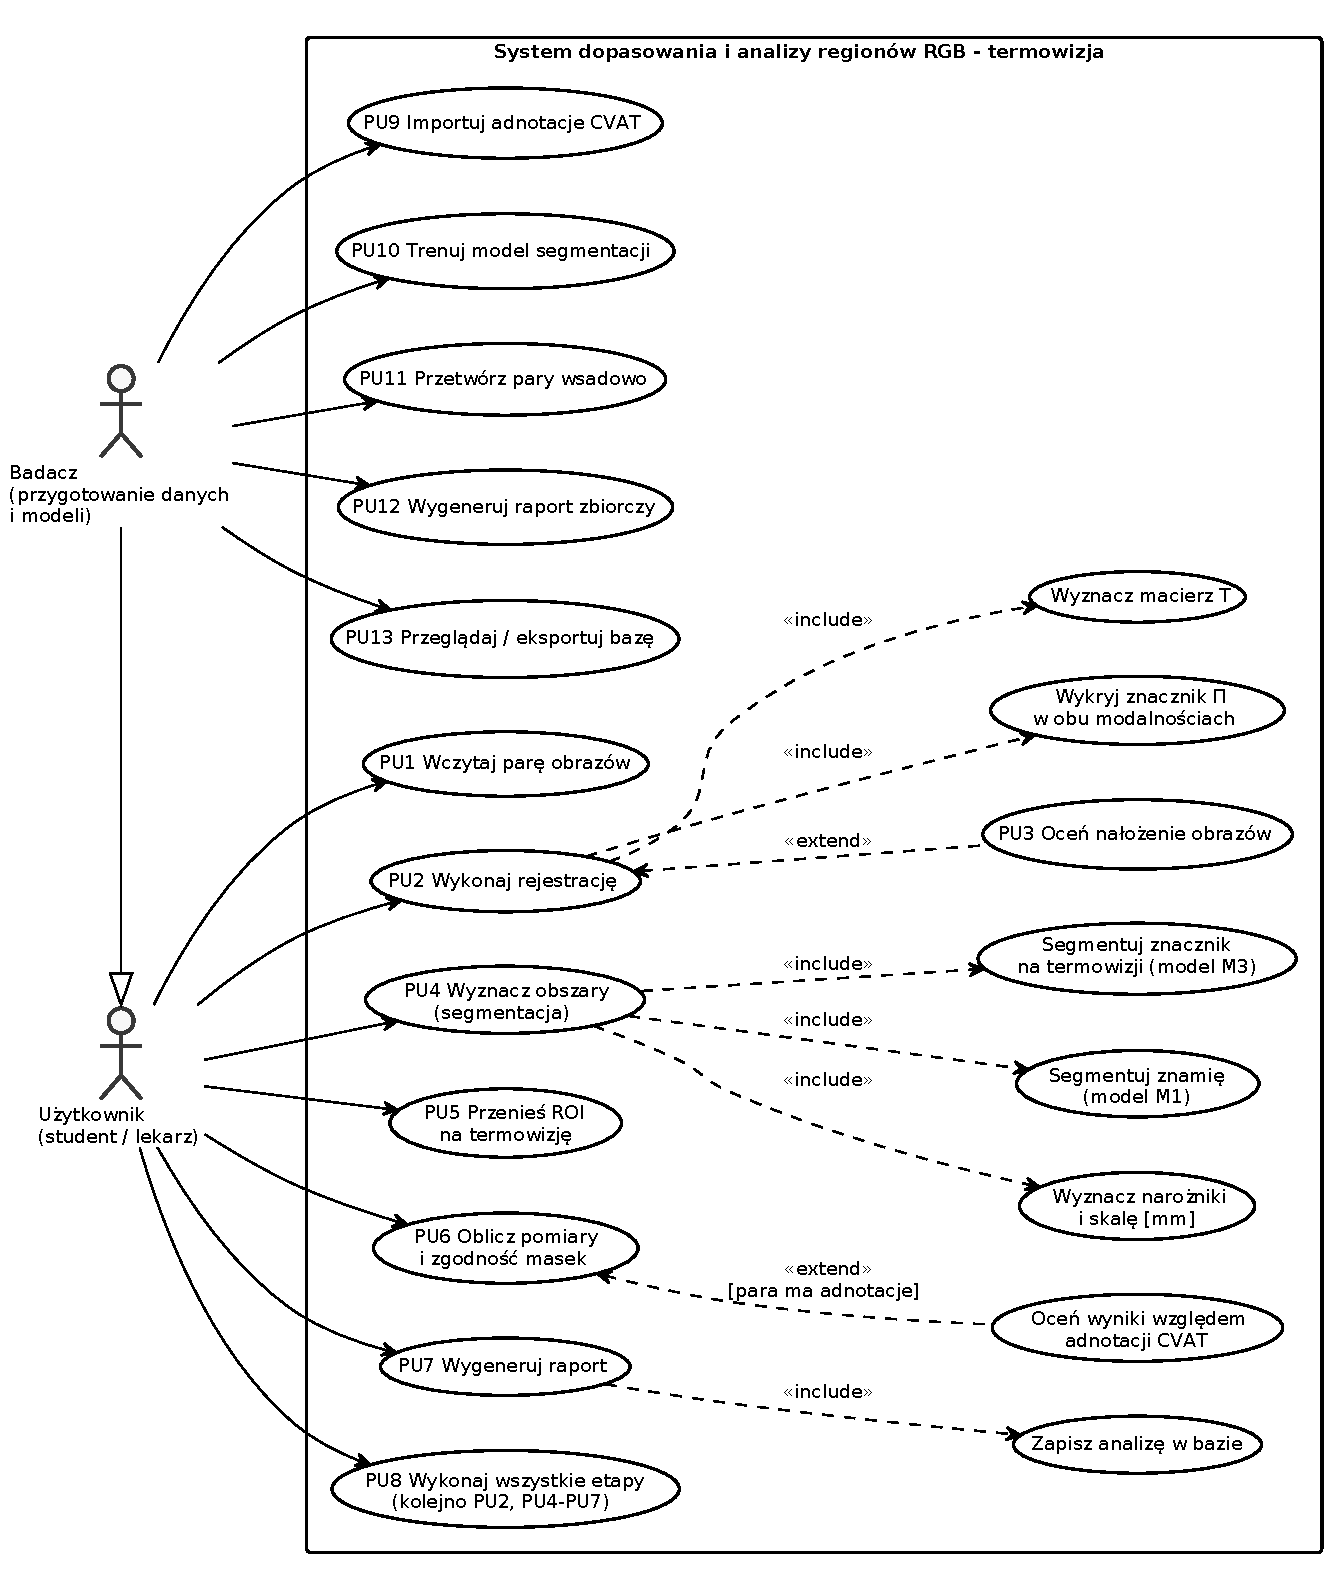
\includegraphics[width=0.85\textwidth]{rysunki/przypadki_uzycia.pdf}
  \caption{Diagram przypadków użycia systemu}
  \label{fig:przypadki-uzycia}
\end{figure}

Przypadek PU2 obejmuje (relacja \guillemotleft include\guillemotright) wykrycie znacznika w obu modalnościach i wyznaczenie macierzy $T$, a ocena nałożenia obrazów (PU3) stanowi jego opcjonalne rozszerzenie (relacja \guillemotleft extend\guillemotright). Ocena wyników względem adnotacji rozszerza przypadek PU6 wyłącznie wtedy, gdy para obrazów ma adnotacje. Scenariusz przypadku PU2 przedstawiono w tabeli~\ref{tab:scenariusz}.

\begin{table}[htbp]
  \centering
  \caption{Scenariusz przypadku użycia PU2 „Wykonaj rejestrację”}
  \label{tab:scenariusz}
  \small
  \begin{tabularx}{\textwidth}{>{\raggedright\arraybackslash}p{3.2cm} X}
    \toprule
    Aktor & Użytkownik \\
    Warunki początkowe & wczytano parę obrazów (PU1) \\
    Scenariusz główny & 1.~Użytkownik wybiera polecenie rejestracji. 2.~System wykrywa znacznik na obrazie termowizyjnym i na zdjęciu. 3.~System wyznacza wstępne dopasowanie kształtów znacznika. 4.~System doprecyzowuje transformację i wybiera jej model. 5.~System wyświetla nałożenie obrazów i zapisuje macierz $T$. \\
    Scenariusze alternatywne & 2a.~Znacznik nie zostaje wykryty -- system wyświetla komunikat i kończy przypadek. 2b.~Kształt wykrytego obiektu słabo odpowiada wzorcowi -- system wyświetla ostrzeżenie. 4a.~Homografia jest niestabilna -- system wybiera przekształcenie afiniczne. \\
    Warunki końcowe & macierz $T$ jest dostępna dla kolejnych etapów \\
    \bottomrule
  \end{tabularx}
\end{table}

\section{Architektura systemu}
\label{sec:architektura}

System zaprojektowano w architekturze potokowej, w której każdy etap korzysta z wyników poprzedniego (rys.~\ref{fig:potok}). Po wczytaniu pary obrazów system wyznacza macierz rejestracji, następnie -- niezależnie od siebie -- narożniki znacznika i skalę, maskę znamienia na zdjęciu oraz maskę znacznika na obrazie termowizyjnym. Kolejne etapy to przeniesienie obszarów przez macierz $T$, pomiary i ocena zgodności oraz raport.

\begin{figure}[htbp]
  \centering
  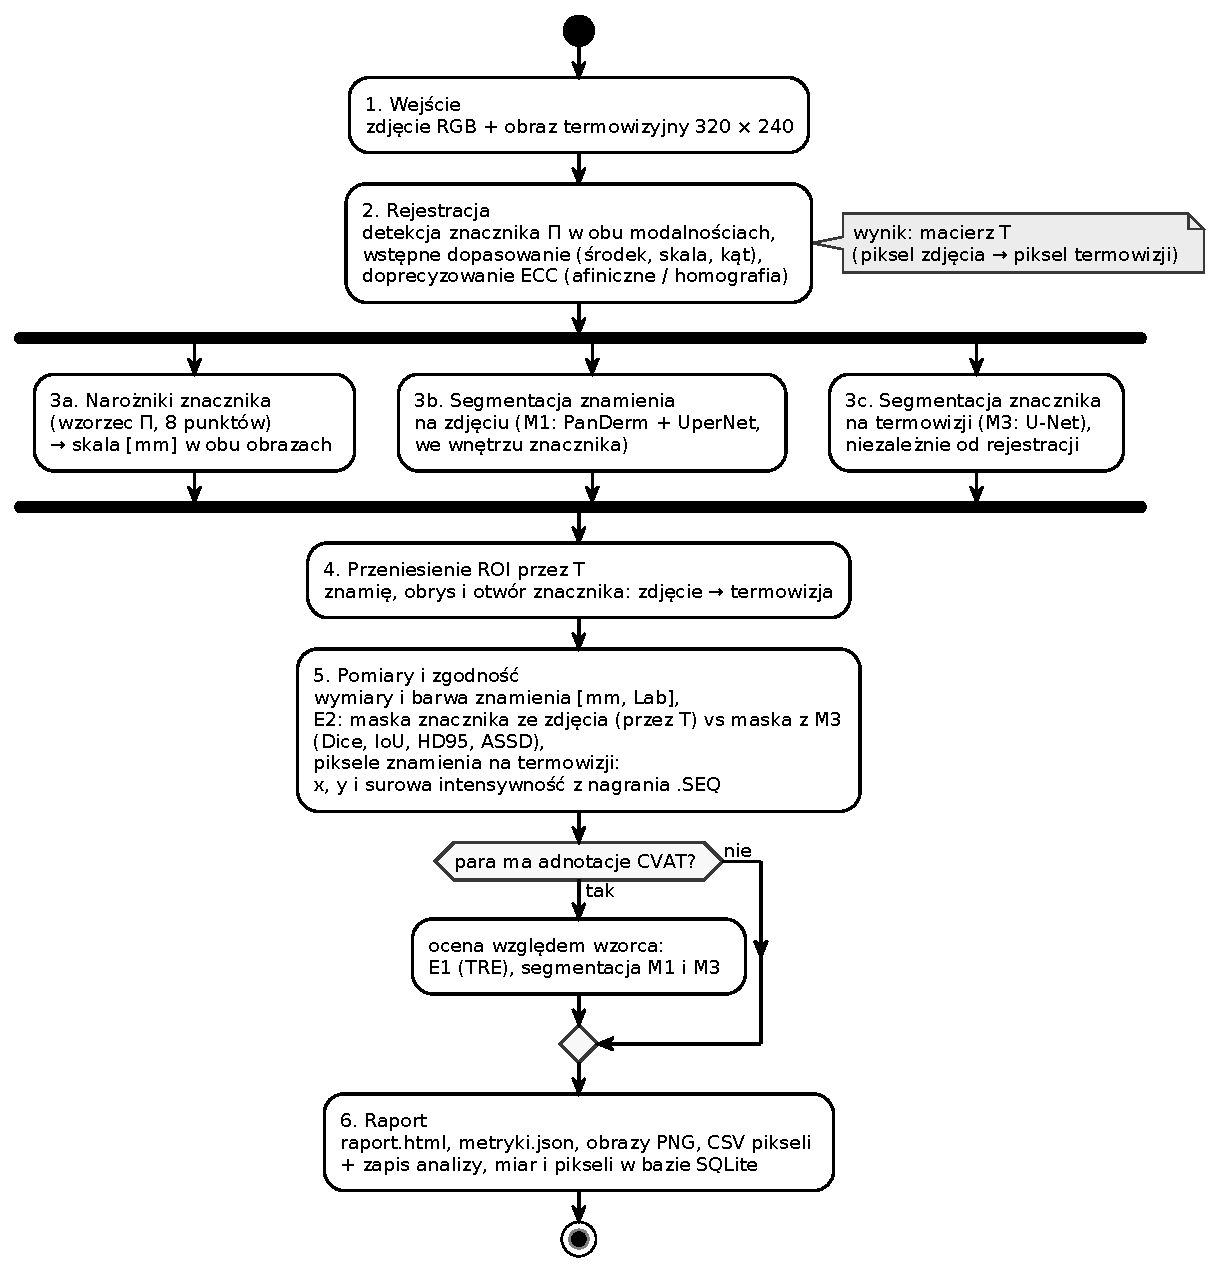
\includegraphics[width=0.6\textwidth]{rysunki/potok_przetwarzania.pdf}
  \caption{Potok przetwarzania pary obrazów (diagram aktywności UML)}
  \label{fig:potok}
\end{figure}

Podział systemu na warstwy przedstawiono na rysunku~\ref{fig:architektura}. Warstwę prezentacji tworzą aplikacja okienkowa i skrypty przetwarzania wsadowego. Obie korzystają z warstwy logiki, w której etapy potoku realizuje jedna klasa, dzięki czemu ten sam kod jest wykorzystywany zarówno w trybie interaktywnym, jak i wsadowym (WN8). Moduły obliczeniowe odpowiadają za rejestrację, segmentację znacznika na obrazie termowizyjnym, przeniesienie obszarów i pomiary oraz raport. Model segmentacji znamienia działa w osobnym środowisku z biblioteką PyTorch i jest uruchamiany jako odrębny proces, co pozwala zachować lekkie środowisko aplikacji (WN7). Warstwę danych tworzą pliki obrazów, masek i wyników, wagi modeli oraz baza danych przechowująca wyniki analiz.

\begin{figure}[htbp]
  \centering
  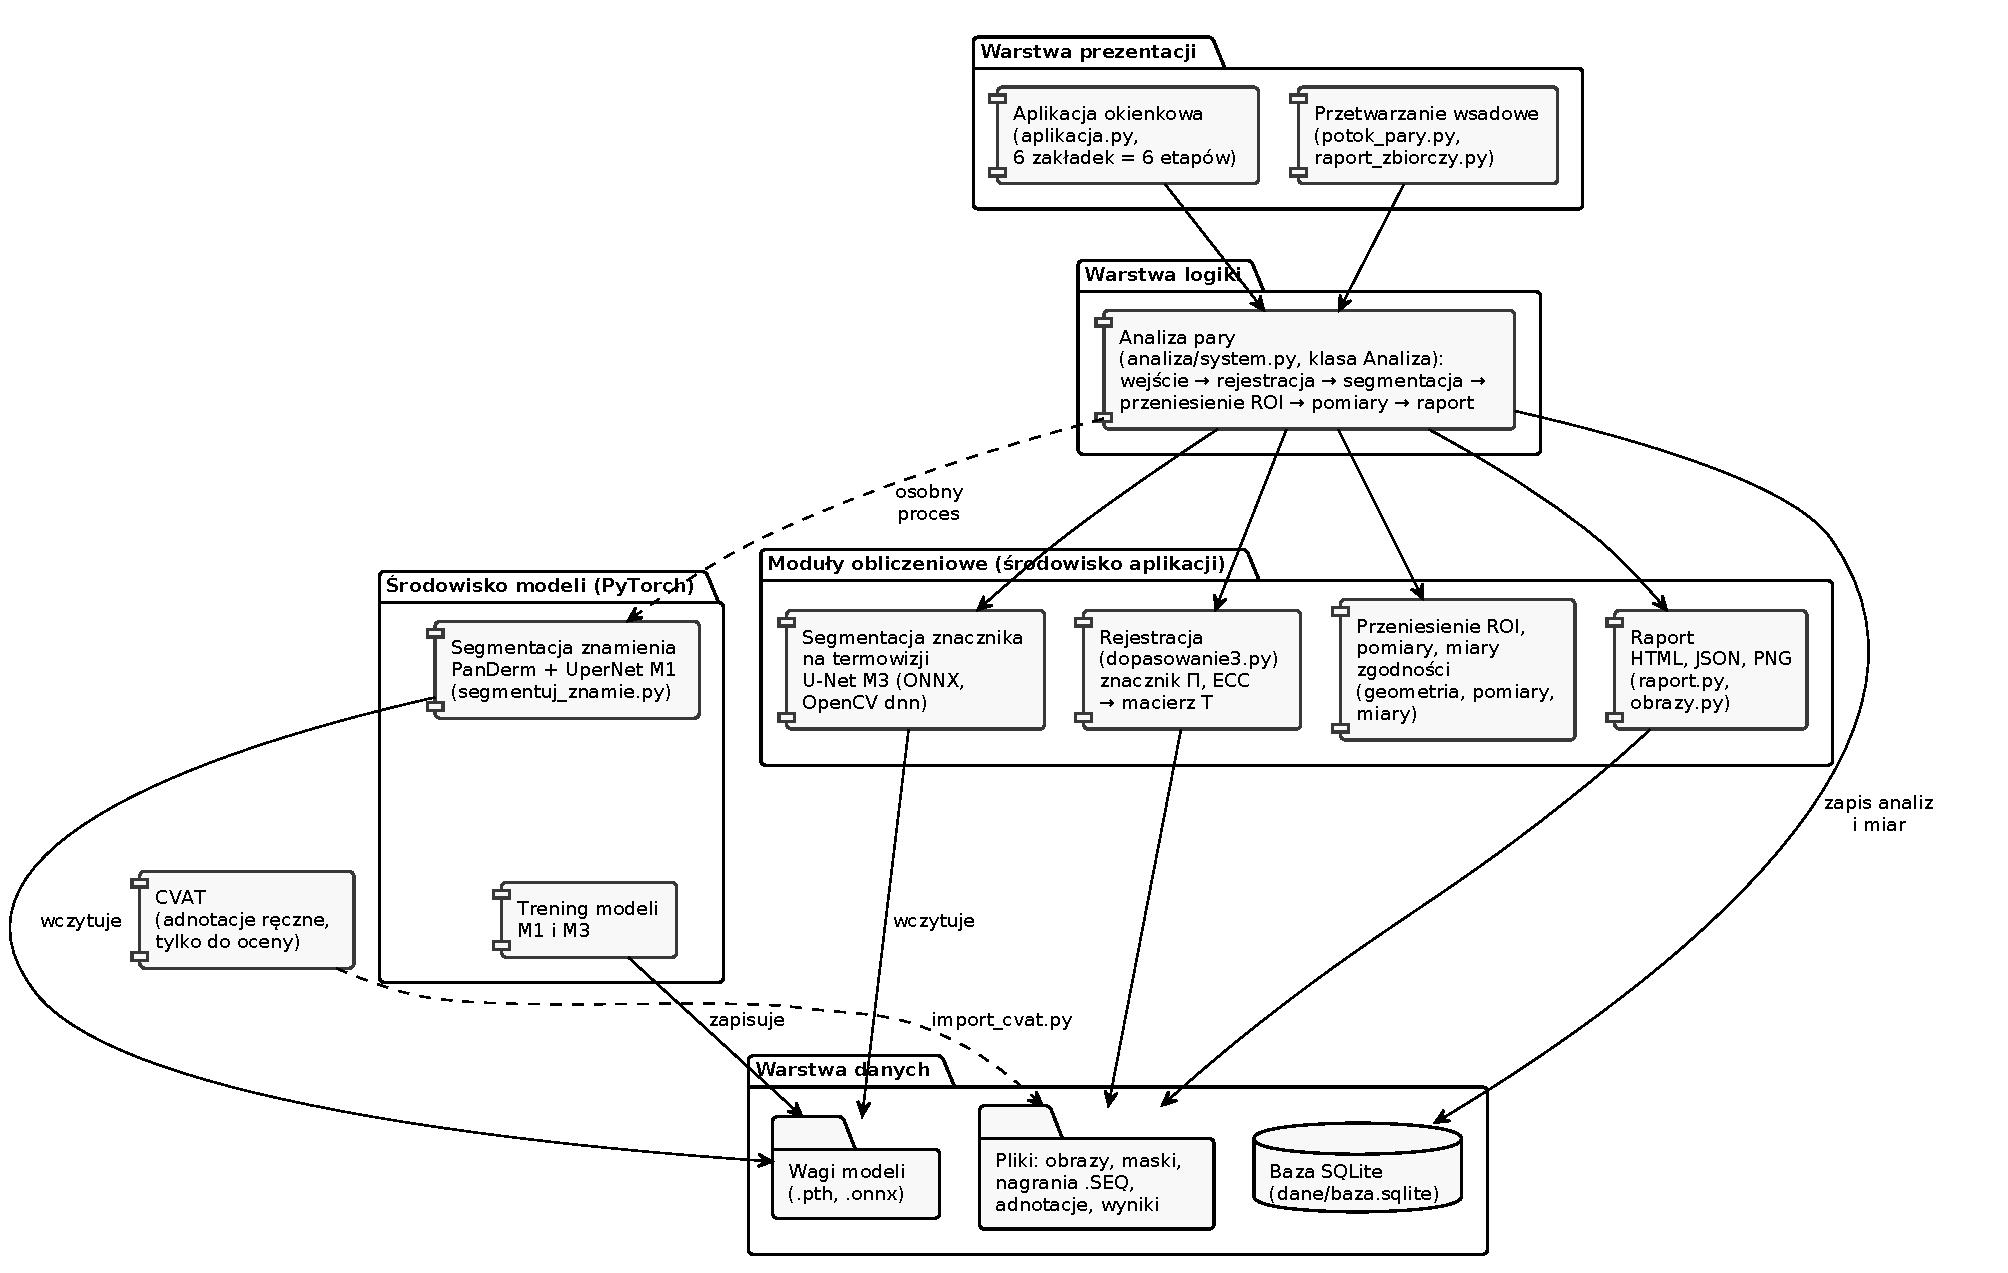
\includegraphics[width=\textwidth]{rysunki/architektura_systemu.pdf}
  \caption{Architektura systemu: warstwy, moduły obliczeniowe i środowiska uruchomieniowe}
  \label{fig:architektura}
\end{figure}
